\documentclass[11pt]{article}
\usepackage[T1]{fontenc}
\usepackage[utf8]{inputenc}
\usepackage{lmodern,microtype}
\usepackage[margin=1in,headheight=15pt]{geometry}
\usepackage{amsmath,amssymb,amsthm,mathtools}
\usepackage{booktabs,array,longtable,enumitem}
\usepackage{xcolor,hyperref,xurl,fancyhdr,listings,tikz}
\usetikzlibrary{arrows.meta,positioning}
\definecolor{ink}{RGB}{30,58,76}
\hypersetup{colorlinks=true,linkcolor=ink,citecolor=ink,urlcolor=ink,
 pdftitle={Cographic Persistence and Causal Reset Complexity for Compressed Unknot Hierarchies},
 pdfauthor={Research continuation prepared for the ProveIt project}}
\pagestyle{fancy}\fancyhf{}
\fancyhead[L]{\small Cographic persistence and causal resets}
\fancyhead[R]{\small ProveIt research continuation}
\fancyfoot[C]{\thepage}
\setlength{\parskip}{0.35em}
\setlength{\parindent}{1.1em}
\setlength{\emergencystretch}{3em}
\setlist{itemsep=0.3em,topsep=0.4em}
\lstset{basicstyle=\ttfamily\small,breaklines=true,columns=fullflexible,showstringspaces=false,
 frame=single,framerule=0.25pt,xleftmargin=0.5em,xrightmargin=0.5em}
\newtheorem{theorem}{Theorem}[section]
\newtheorem{lemma}[theorem]{Lemma}
\newtheorem{proposition}[theorem]{Proposition}
\newtheorem{corollary}[theorem]{Corollary}
\theoremstyle{definition}
\newtheorem{definition}[theorem]{Definition}
\newtheorem{example}[theorem]{Example}
\newtheorem{remark}[theorem]{Remark}
\newcommand{\Z}{\mathbb Z}
\newcommand{\Q}{\mathbb Q}
\newcommand{\F}{\mathbb F}
\newcommand{\cut}{\mathbin{\backslash\!\backslash}}
\newcommand{\rank}{\operatorname{rank}}
\newcommand{\comp}{\operatorname{cc}}
\newcommand{\poly}{\operatorname{poly}}
\newcommand{\supp}{\operatorname{supp}}
\newcommand{\code}[1]{\texttt{\detokenize{#1}}}
\newcommand{\parents}{\operatorname{par}}
\newcommand{\children}{\operatorname{ch}}
\newcommand{\bits}{\operatorname{bits}}
\begin{document}
\begin{titlepage}
\vspace*{0.3in}
{\large\sffamily\color{ink} TOPOLOGY / UNKNOT RECOGNITION\par}
\vspace{0.28in}
{\LARGE\bfseries Cographic Persistence and\par
Causal Reset Complexity\par}
\vspace{0.13in}
{\Large for Compressed Unknot Hierarchies\par}
\vspace{0.25in}
{\large Optimal reuse of nonseparating cuts, one-census chamber graphs,\par
and a downstream-amplified spanning-tree principle\par}
\vspace{0.3in}
{Research continuation prepared for Vladimir Reshetnikov's ProveIt project\par}
{12 October 2026\par}
\vspace{0.24in}
\begin{abstract}
A compressed local operation does not by itself control the repeated destruction and reconstruction of later hierarchy work. We develop a certificate-based approach to this reset bottleneck. For a source-authenticated system of connected, disjoint, cooriented surfaces, we recover its chamber graph from one scalar weighted-orbit census. The nonseparating subbatches are exactly the independent sets of the cographic matroid. A minimum-weight spanning tree therefore selects an optimal batch, while a shared routing forest supplies dual-loop descriptions in an explicit finite source arena.

The geometric certificate is a surface together with a loop crossing it once and avoiding the other retained surfaces. We prove precisely which local modifications preserve these witnesses. We then analyze a fixed acyclic graph of genuine certificate dependencies. If a task has rebuild cap $g_i$ and initial remaining potential $d_i$, its number of version changes is bounded by
\[
 B_i=d_i+(g_i+1)\sum_{j\to i}B_j.
\]
The bound expands as a weighted sum over directed paths and is sharp on chains. An eventwise potential also accounts for unobserved parent changes and explicitly charges changes of dependency arena. A reverse recurrence computes the downstream cost of lost progress. Combining these costs with the chamber graph gives an exact minimum-spanning-tree rule for minimizing the resulting certified restart bound.

The contribution includes proofs, a standard-library reference implementation, independent verifiers, exhaustive and randomized finite checks, and paired graph-stage measurements. It does not establish a general quasi-polynomial unknot recognizer. In particular, an initial knot exterior permits a nonseparating batch of size at most one. The remaining challenge is to realize source-authenticated persistence with small actual causal depth, controlled encoded geometry, and the original hierarchy's correctness obligations intact.
\end{abstract}
\vfill
{\small\textbf{Status.} Topological, graph, and reset-model results are proved here. The end-to-end recognition bound is conditional. Native ProveIt geometry and full recognition were not executed in this study.}
\end{titlepage}
\tableofcontents
\clearpage

\section{The target: stop discarding independent hierarchy work}
\subsection{The inspected checkpoint}
The maintained ProveIt recognizers do not have a proved general quasi-polynomial bound \cite{repo}. The inspected raw-cut construction retains all cell dimensions, signed incidences, and reconstruction charts in binary affine families. Its representation distinguishes a geometric attaching map from the much weaker data of a cellular boundary matrix \cite{cutcells}. This is the right foundation for persistent certificates: one must know \emph{where} a witness lives, not merely which scalar invariant it contributes.

Lackenby's hierarchy algorithm supplies a particularly relevant target. Its Section~9 analyzes a restart process with hierarchy-length bound $L$ and surface pattern-complexity bound $g$, obtaining the iteration bound $L(g+1)^L$. A simplification of an earlier surface can discard its suffix. The refined construction bounds hierarchy length linearly in initial q-complexity, rather than logarithmically. Individual running-time bounds remain separate obligations \cite[Sections~9--10]{lackenby}.

The research question is therefore not simply whether normal coordinates can be made small. It is:
\begin{quote}
Can a verified change invalidate only the certificates that actually depend on it, and can the resulting dependency structure have much smaller depth than the stored hierarchy?
\end{quote}
This paper provides a precise mathematical model and several geometric prerequisites for answering that question. It does not silently replace an existing hierarchy by an arbitrary reordered list of surfaces.

\subsection{Three layers of the contribution}
The first layer is \emph{simultaneous nonseparation}. Two disjoint surfaces can each be nonseparating while their union separates. We characterize all valid subbatches by a finite graph, recover that graph with a single weighted census, and optimize additive retention rewards without subset enumeration.

The second layer is \emph{witness persistence}. A dual loop is a constructive certificate of nonseparation. Its support must be included in the read set of a retained surface. We prove a local preservation statement and distinguish it from unproved preservation of global properties such as incompressibility or boundary-pattern essentiality.

The third layer is \emph{causal accounting}. A task can be rebuilt only after a genuinely new parent version. The relevant complexity is a sum over dependency paths. Long lists with independent entries have no multiplicative reset penalty; long dependency chains can still have exponential penalties. Reverse path weights connect this model back to optimal geometric batch selection.

\subsection{Attribution and the novelty boundary}
The dual graph of a disjoint hypersurface system, graph cycle lattices, cographic matroids, and spanning-tree optimization are classical. Their elementary proofs are included because the exact integral and source-labeling conditions matter to the proposed algorithm. We do not claim these foundations as new discoveries. Weighted interval-orbit counting is imported from Agol--Hass--Thurston \cite[Theorem~16]{aht}, not reimplemented here.

The proposed research contribution is their combination into a one-census, proof-carrying persistence operator, together with the explicit reset recurrence and its downstream-amplified reuse objective. Priority for this combination has not been established by an exhaustive literature search. The inspected incoming first-return and boundary-kernel excerpts concern related compressed interfaces; we do not assume that they supply the source-local persistence or fixed-DAG accounting developed below \cite{moment,corners,sparse}. Earlier ProveIt ``closure resets'' concern Khovanov scanning, while earlier causal RIII work concerns local diagram rewrites; neither is the hierarchy version model studied here \cite{closures,causalr3}.

\section{Geometric and computational conventions}
\subsection{A labeled system is more than a normal vector}
Throughout Sections~\ref{sec:duality}--\ref{sec:persistence}, $M$ is a connected compact orientable piecewise-linear $3$-manifold, possibly with boundary. A \emph{candidate system}
\[
\mathcal S=(S_1,\ldots,S_k)
\]
consists of nonempty connected compact properly embedded surfaces. They are pairwise disjoint and two-sided, with chosen coorientations. Their collars are pairwise disjoint. Corners created by cutting are rounded without changing the relevant topology.

These hypotheses must be authenticated by the geometric caller. A list of normal vectors that passes quadrilateral compatibility is not, by itself, a certificate that the claimed labeled components have been coembedded as this particular disjoint system. One must retain the common source, the component labels, and the side labels. One-sided surfaces and disconnected ``surfaces'' represented by a single edge are outside this interface.

Write $M\cut\mathcal S$ for cutting along all candidate surfaces and $M_J=M\cut\bigcup_{j\in J}S_j$ for a subbatch $J\subseteq\{1,\ldots,k\}$. A subbatch is \emph{valid} in this paper when $M_J$ is connected. This word asserts only nonseparation, not admissibility as a complete essential-hierarchy step.

\subsection{The chamber graph}
The vertices of $G=G(M,\mathcal S)$ are the connected components of $M\cut\mathcal S$. Each candidate surface supplies one oriented edge $e_i$, from the chamber containing its negative side to the chamber containing its positive side. The two chambers may coincide, and different surfaces may supply parallel edges. Connectivity ignores the chosen orientations.

Let $c=|V(G)|$. Since $M$ is connected, $G$ is connected: reattaching all collars reconstructs a connected manifold, and its components are exactly described by the connectivity of the graph. In particular,
\begin{equation}\label{eq:chamber-size}
 c\leq k+1.
\end{equation}
This graph is not a planar dual graph and need not be planar. No planar separator or sphere-boundary premise is involved.

\subsection{Input size and the trusted boundary}
For graph algorithms, a graph with $c$ vertices, $k$ edges, and maximum reward bit length $W$ has $O(k(W+\log(k+2)))$ encoded bits. We use nonnegative integer rewards and account for their bit lengths.

For compressed geometry, let $Q$ denote the number of source records and $B$ the largest source-index or coordinate bit length. An encoded namespace may contain $N$ cells with $\log(N+1)=O(B+\log(Q+1))$, while $N$ itself is enormous. An operation polynomial in $N$ is not considered compressed. The source-to-orbit translation and its verification must be charged separately from the short graph computation.

The reference code accepts graph-level and finite-arena facts. It never promotes their verification into a claim that an input is a triangulated manifold, a valid normal surface, or an unknot. The maintained raw-cut source has a narrower geometric input domain than the abstract theorems here; a later-piece adapter needs its own validation.

\section{Integral duality and exact nonseparating batches}\label{sec:duality}
Let $\partial_G:\Z^k\to\Z^c$ be the oriented incidence map: an edge from $u$ to $v$ maps to $v-u$. Loops map to zero. Coorientation defines a homomorphism
\[
 I:H_1(M;\Z)\longrightarrow\Z^k,
 \qquad I([\gamma])=(\gamma\cdot S_1,\ldots,\gamma\cdot S_k),
\]
where a transverse closed curve is counted with signed intersections. The individual coordinate homomorphisms are denoted $\alpha_i\in H^1(M;\Z)$.

\begin{theorem}[Integral chamber-cycle theorem]\label{thm:lattice}
For a candidate system as above,
\begin{equation}\label{eq:cycle-image}
 I(H_1(M;\Z))=\ker\partial_G.
\end{equation}
Thus the image is a saturated free sublattice of $\Z^k$ of rank $k-c+1$. The induced surjection $H_1(M;\Z)\twoheadrightarrow H_1(G;\Z)$ splits as a homomorphism of abelian groups. In particular,
\[
 \rank\langle\alpha_1,\ldots,\alpha_k\rangle=k-c+1.
\]
\end{theorem}
\begin{proof}
Move a representative integral one-cycle into the interior of $M$ and make it transverse to the surfaces. Following it records a sequence of chamber visits and signed collar crossings. At each chamber the algebraic number of entries equals the algebraic number of exits. Therefore $\partial_G I([\gamma])=0$.

Conversely, every integral graph cycle is an integral sum of closed oriented walks. To lift one such walk, choose an interior point of each surface whenever its edge is traversed, cross the collar in the required direction, and join consecutive crossing endpoints by paths in the intervening chamber. These joining paths exist because that chamber is connected and a manifold is locally path connected. Their interiors avoid every cut surface. Closing the last path gives a loop in $M$ whose intersection vector is the graph cycle. Repeated occurrences are permitted at this stage. Summing these loops proves surjectivity onto $\ker\partial_G$.

For a connected graph, a spanning tree shows directly that the incidence map has rank $c-1$: its tree columns are independent, and every column has total coordinate sum zero. Consequently its kernel has rank $k-c+1$. The kernel of a homomorphism between free abelian groups is saturated when its quotient is the image, which here is a subgroup of the torsion-free group $\Z^c$. Choose lifts in $H_1(M;\Z)$ of a free basis of this kernel to split the surjection. Finally the rank of the intersection map equals the rank of the span of its coordinate functionals, giving the last assertion.
\end{proof}

\begin{remark}
Equation~\eqref{eq:cycle-image} is stronger than a rational rank test. Fundamental graph cycles give integral witnesses with coefficients $0,1,-1$, and the nonseparating batch witnesses below have an identity intersection matrix. Torsion in $H_1(M;\Z)$ cannot create a hidden denominator in these certificates.
\end{remark}

\begin{theorem}[Subbatch connectivity and homological rank]\label{thm:subbatch}
For every $J\subseteq\{1,\ldots,k\}$,
\begin{equation}\label{eq:components}
 \comp(M_J)=\comp(G-\{e_j:j\in J\})
 =1+|J|-\rank\langle\alpha_j:j\in J\rangle.
\end{equation}
Consequently $J$ is valid exactly when $G-J$ is connected, or equivalently when the classes $\{\alpha_j:j\in J\}$ are linearly independent over $\Q$.
\end{theorem}
\begin{proof}
Start with the fully cut manifold. Reattach just the collars of the surfaces outside $J$. This joins chambers along precisely the edges outside $J$, so its connected components are the components of $G-J$. The resulting manifold is $M_J$.

Alternatively, consider the dual graph for the smaller system $(S_j)_{j\in J}$. Its vertices are those components, and its edges are the surfaces in $J$. Theorem~\ref{thm:lattice} for this smaller system gives the rank $|J|-\comp(M_J)+1$ of its intersection map. Its coordinate functionals are exactly the original $\alpha_j$, so rearrangement gives the second equality.
\end{proof}

\begin{corollary}[The cographic batch structure]\label{cor:cographic}
The valid subbatches are the independent sets of the cographic matroid of $G$. Their maximum cardinality is $k-c+1$. Every subset of a valid batch is valid, and its cuts may be performed in any order without making a later member separating.
\end{corollary}
\begin{proof}
One definition of cographic independence is that deleting the chosen edges leaves a connected graph. A maximum independent set is the complement of a spanning tree. For a valid batch, every partial batch is valid by adding back some deleted edges. After a prefix has been cut, the next surface has connected cut complement by applying Theorem~\ref{thm:subbatch} to the enlarged prefix.
\end{proof}

\begin{corollary}[The initial knot-exterior barrier]\label{cor:knot-barrier}
If $M$ is a knot exterior in $S^3$, every valid candidate subbatch has at most one member.
\end{corollary}
\begin{proof}
Let $V$ be the closed tubular solid torus of the knot, with common boundary $T$. Mayer--Vietoris for $S^3=M\cup V$ gives an isomorphism
\[
 H_1(T;\Z)\cong H_1(M;\Z)\oplus H_1(V;\Z),
\]
because $H_2(S^3;\Z)=H_1(S^3;\Z)=0$. Since the left side is $\Z^2$ and $H_1(V;\Z)=\Z$, the direct summand $H_1(M;\Z)$ is free of rank one. The independent intersection functionals in a valid batch therefore number at most one.
\end{proof}
This is a real restriction, not an implementation inconvenience. The persistence program must obtain its larger opportunities in later pieces, in independently certified local work, or in a representation more general than simultaneous nonseparating cuts in the initial exterior. The corollary does not bound the length of a sequential hierarchy: surfaces created after a cut need not be simultaneously disjoint properly embedded surfaces in the original exterior.

\begin{example}[Parallel meridian disks]\label{ex:meridians}
Two parallel meridian disks in a solid torus are disjoint and individually nonseparating. Cutting along both produces two balls. The chamber graph has two vertices and two parallel edges, so either singleton is valid but the pair is not. This example refutes the rule ``keep all disjoint nonseparating surfaces'' even for the exterior of the unknot.
\end{example}

\section{Recovering the chamber graph with one scalar census}\label{sec:census}
\subsection{The source contract}
Suppose a validated compressed raw cut supplies a finite atomic chamber namespace $\Omega$ and a compressed equivalence relation generated by identifications through original-face regions. Its equivalence classes must be exactly the connected components of $M\cut\mathcal S$. Identifications crossing the candidate surfaces are \emph{not} included.

For each $S_i$, the source also supplies an atom $a_{2i-2}$ incident to its negative side and an atom $a_{2i-1}$ incident to its positive side. Because a side of a connected two-sided surface is connected, it lies in a unique global chamber. Thus a single marked atom determines the chamber of that entire side. Different markers may be attached to the same atom.

\begin{lemma}[No unmarked chamber]\label{lem:marked}
If $k>0$, every equivalence class in the authentic chamber relation contains at least one of the $2k$ side markers.
\end{lemma}
\begin{proof}
Every vertex of a connected graph with at least one edge is incident to an edge, allowing loops. Apply this to the chamber graph. The marker on the corresponding connected side is in that chamber.
\end{proof}

\subsection{The compiler}
Assign to each atom the nonnegative scalar weight
\begin{equation}\label{eq:marker-weight}
 w(a)=\sum_{\{j:a_j=a\}}2^j,\qquad 0\leq j<2k,
\end{equation}
with zero weight at all other atoms. Aliases are combined by \emph{addition}; overwriting a previous marker is incorrect. Run one weighted-orbit census and record the orbit-weight histogram. An authentic output has one row $(m_C,1)$ for each chamber $C$, where
\[
 m_C=\sum_{a_j\in C}2^j.
\]
The powers of two are unique globally, so these are disjoint bit masks, not a numerical approximation.

\begin{theorem}[One-census chamber compiler]\label{thm:census}
For $k>0$, the histogram above determines the full oriented, edge-labeled chamber graph. It has at most $k+1$ rows, every row has nonzero weight and multiplicity one, and the row masks partition the $2k$ marker bits. Decoding marker $2i-2$ and marker $2i-1$ gives the negative and positive endpoint of $e_i$.

If the source relation is given by a weighted interval-pairing instance with $Q$ generators and maximum index bit length $B$, this construction uses weights of at most $2k$ bits and $O(k)$ constant-weight intervals. Its bit cost is polynomial in $Q,B,k$, using the imported weighted-orbit algorithm. No represented atom is enumerated.
\end{theorem}
\begin{proof}
The unique occurrence of each marker means that summing weights over an orbit puts exactly its marker bits into the resulting integer. Distinct nonempty marker sets have distinct integer values. Lemma~\ref{lem:marked} excludes zero-weight chambers, and hence every row multiplicity is one. All $2k$ bits occur once, because every marker has one source location. Decoding them recovers the endpoints by the source contract. Equation~\eqref{eq:chamber-size} bounds the number of rows.

There are at most $2k$ marked locations. Splitting the linearly indexed namespace at their singleton positions gives $O(k)$ constant-weight intervals, including zero-weight gaps. The largest weight and the sum of the distinct marker weights are below $2^{2k}$. The weighted interval-orbit theorem therefore has polynomial dependence on the generator count, the number of intervals, $\log(N+1)$, and $k$ \cite{aht}. Sparse marker preparation and bit-mask decoding also have polynomial bit cost. This proves the stated bound subject to the source-to-pairing contract.
\end{proof}

\paragraph{The empty case.} For $k=0$ the graph has one vertex and no edges. The correct histogram convention is the single row $(0,1)$. A generic prohibition on zero-weight rows must not reject this case.

\paragraph{Consistency is not source authentication.} The decoder checks coverage, disjoint masks, multiplicity, connectivity, and endpoint range. A fabricated histogram can pass all these checks. It is still not a proof about a manifold. The independent source-orbit verifier must authenticate the underlying relation and all marker placements before the graph can be used geometrically.

\paragraph{An alias example.} Suppose markers $0,1,3$ occupy atom $17$ and marker $2$ occupies atom $3$, and the two atoms are in different chambers. The histogram is $(11,1),(4,1)$. The first candidate is a loop at the first chamber; the second joins the second chamber to the first. There are only two nonzero source locations, despite four markers. This exact case is tested in the implementation.

\subsection{What the census does not export}
The census identifies the chamber containing a source atom. It need not return a short path between two atoms in that chamber. Such paths are needed to locate dual-loop witnesses in actual source geometry. It is not legitimate to treat a connectedness count as a compressed path certificate. Section~\ref{sec:routing} solves this lift for a finite explicit arena and formulates the additional requirement for binary source families.

The new compiler has a different purpose from first-return recovery on a boundary circle. It marks the two sides of entire connected surfaces and counts \emph{three-dimensional chambers}. Its polynomial output bound comes from $c\leq k+1$, not from a general promise that a compressed namespace has only polynomially many orbits. Here $k$ counts explicitly labeled candidate components. A normal vector representing exponentially many parallel connected components does not automatically provide a small labeled candidate list. The theorem is polynomial in $k$ as well as the source bit size; it does not enumerate an exponential batch for free.

\section{Optimal batch selection and independent verification}\label{sec:selection}
Give each candidate a nonnegative integer reward $w_i$. The objective is to maximize $w(J)=\sum_{i\in J}w_i$ among valid batches.

\begin{theorem}[Optimal nonseparating reuse]\label{thm:mst}
Let $T$ be a minimum-weight spanning tree of the chamber graph. Then
\[
 J=E(G)\setminus T
\]
is a maximum-reward valid batch. Every valid batch can be extended to one of this form without decreasing its reward. After the chamber graph is known, a producer requires $O(k\log(k+2))$ weight comparisons and $O(k)$ records. The supplied independent verifier uses $O(kc)$ graph work and comparisons.
\end{theorem}
\begin{proof}
If $J$ is valid, the connected graph $G-J$ contains a spanning tree $T_J$. Hence $J\subseteq E(G)\setminus T_J$. Nonnegative rewards imply
\[
 w(J)\leq w(E(G))-w(T_J)\leq w(E(G))-w(T).
\]
The complement of $T$ is valid and attains the last expression.

Kruskal's algorithm sorts the edges and adds an edge exactly when it joins two current components. The forest maintained by this procedure can always be extended to a minimum spanning tree: when the next accepted edge is not in a chosen minimum tree extension, insert it and remove a crossing edge on the resulting cycle. The removed edge is no cheaper, by the order in which components were joined. Induction proves optimality. A disjoint-set structure gives the stated comparison and storage bounds.

The certificate contains the graph, its rewards, the selected tree, and its complement. The independent checker verifies that the tree spans and has $c-1$ edges, that the complement and objective are correct, and that each off-tree edge has weight at least the maximum weight on its tree return path. This cycle condition characterizes minimum spanning trees. To see sufficiency, compare with any other spanning tree and repeatedly exchange a missing edge of the certified tree into it; the cycle condition, or the equivalent threshold-component characterization, ensures that a no-cheaper crossing edge can be removed. More explicitly, remove an edge $f$ of the certified tree to define a cut. Every other edge crossing that cut has certified-tree return path containing $f$, and hence has weight at least $w(f)$. If another spanning tree does not contain $f$, its path between the endpoints of $f$ crosses this cut at an edge $e$ outside the certified tree. Inserting $f$ and deleting $e$ does not increase weight and increases the number of shared tree edges. Iterating proves optimality. The checker performs an independent breadth-first path search for each off-tree edge, giving $O(kc)$ work.
\end{proof}

\paragraph{Bit accounting.} The producer's sorting comparisons act on $W$-bit rewards. Summed rewards have $O(W+\log(k+2))$ bits. Both construction and checking are polynomial in the full graph input length. The reference checker intentionally favors a small independent implementation over optimal asymptotic verification. It does not claim linear-time minimum-spanning-tree verification.

\paragraph{Zero rewards, loops, and bridges.} Zero rewards cause ties but no difficulty. A loop can always be selected. A bridge can never be selected, regardless of reward. Negative rewards would require a modified optimization problem and are rejected by the supplied interface.

\begin{proposition}[The abstraction's exact scope]\label{prop:replacement}
Replacing each full-cut chamber by an arbitrary connected chamber with the same labeled side incidences preserves the family of valid subbatches and every additive optimal-batch value. It need not preserve $\pi_1$, homology inside chambers, homeomorphism type, or the knot represented by the entire source.
\end{proposition}
\begin{proof}
The replacement leaves the chamber graph unchanged, so Theorems~\ref{thm:subbatch} and~\ref{thm:mst} apply with identical data. An interior connected sum with a closed nontrivial $3$-manifold changes interior topology without changing any side incidence, demonstrating why stronger conclusions do not follow.
\end{proof}
This is a useful minimality statement for an optimizer: the graph is a sufficient abstraction for this particular query, not a replacement for the source manifold.

\section{Dual loops, shared routing, and local persistence}\label{sec:persistence}
\subsection{Certificates for a whole batch}
\begin{theorem}[Disjoint dual-loop certificates]\label{thm:loops}
A batch $J$ is valid if and only if there exist closed embedded curves $\gamma_j$ in the interior of $M$, for $j\in J$, such that $\gamma_j$ meets $S_j$ transversely once with positive sign and is disjoint from every $S_i$ with $i\in J\setminus\{j\}$. The curves can be chosen pairwise disjoint. Consequently the sets $S_j\cup\gamma_j$ have pairwise disjoint regular neighborhoods.
\end{theorem}
\begin{proof}
Suppose $J$ is valid. Choose a spanning tree $T\subseteq G-J$. For each selected edge $e_j$, traverse $e_j$ positively and return along the unique tree path. This fundamental closed walk contains no other selected edge. Lift it to $M$ as in Theorem~\ref{thm:lattice}. The chosen loop crosses $S_j$ exactly once, and avoids all other selected surfaces. Tree edges may correspond to unselected surfaces, which the loops are allowed to cross.

The lifts can be made embedded and mutually disjoint by general position for finitely many one-dimensional curves in a three-manifold, relative to small prescribed crossing neighborhoods. Within chambers, perturb their finitely many arcs off each other; in surface collars choose distinct crossing points. This does not create crossings with a selected surface that was previously avoided. Pairwise disjoint compact sets admit pairwise disjoint sufficiently small regular neighborhoods.

Conversely, the intersection matrix $(\gamma_j\cdot S_i)_{j,i\in J}$ is the identity. The functionals $\alpha_i$ are therefore independent. Theorem~\ref{thm:subbatch} implies validity.
\end{proof}

\subsection{The finite source-arena lift}\label{sec:routing}
A finite arena is a graph on $N_0$ atomic chambers with two types of edges. \emph{Interior edges} join atoms across source interfaces without crossing a candidate surface. For each candidate surface there is exactly one oriented \emph{gate} joining its selected negative-side atom to its selected positive-side atom. The connected components of the interior graph are the global chambers. Source charts must justify this interpretation; the arena alone is combinatorial.

\begin{proposition}[One routing tree for all selected witnesses]\label{prop:routing}
Choose a spanning tree in each interior component and a chamber spanning tree $T$. The union of the interior trees and the gates indexed by $T$ is a spanning tree of the full arena. Each gate outside $T$, together with its tree return path, gives a dual-loop description crossing exactly one selected gate. All descriptions share $O(N_0+k)$ tree-and-chord records.
\end{proposition}
\begin{proof}
If there are $c$ interior components, their spanning forest contains $N_0-c$ edges. Adding the $c-1$ gates of the chamber tree joins these components without a cycle. The result is connected with $N_0-1$ edges, hence a tree. The fundamental cycle of any remaining gate uses that gate once and no other non-tree gate. Store the common tree once and identify each cycle by its chord. This requires $N_0-1$ tree edges and at most $k$ chord identifiers, rather than storing each return path separately.
\end{proof}
Explicit expansion of all paths can still cost $\Theta(kN_0)$. The shared description is a graph-level certificate, and geometric disjointification from Theorem~\ref{thm:loops} is not performed by this reference module. On a binary family namespace, even storing one forest edge per atom may be exponentially large. A compressed path grammar with authenticated support is a separate construction problem; the finite result must not be relabeled as its solution.

\begin{proposition}[Topological realization of the graph fixtures]\label{prop:realization}
Every finite connected multigraph is the chamber graph of a system of connected cooriented disks in an orientable handlebody.
\end{proposition}
\begin{proof}
Take one $3$-ball for each vertex. For each edge attach a $1$-handle between small disjoint boundary disks of its endpoint balls; for a loop, use two boundary disks on the same ball. Coorient the co-core disk of each $1$-handle. Cutting along all co-cores leaves the vertex balls with half-handle collars, still balls. Its chamber graph is the original multigraph. The connected union is a handlebody, as can also be seen by first adding the handles of a graph spanning tree and then the remaining handles.
\end{proof}
Thus the graph examples have genuine topological realizations. This observation is not a claim that the supplied tests built or cut their triangulations.

\subsection{What survives a local change}
\begin{theorem}[Local persistence of nonseparation]\label{thm:persistence}
Let $S$ have a dual-loop witness $\gamma$ meeting it exactly once. Suppose a modification produces an orientable manifold $M'$ and leaves an authenticated neighborhood of $S\cup\gamma$ unchanged, as an embedded neighborhood with $S$ still proper. Then the transported $S$ is nonseparating in the connected component of $M'$ containing it.

More generally, suppose a compression or boundary-compression surgery on $S$ is supported away from $\gamma$, leaves the unique crossing point unchanged, and produces a two-sided properly embedded surface $S'$. Exactly one component $S'_0$ of $S'$ meets $\gamma$, it meets it once, and $S'_0$ is nonseparating in its ambient component. For a batch of disjoint witnessed surfaces, all other witnesses whose full neighborhoods are untouched remain valid.
\end{theorem}
\begin{proof}
A separating two-sided surface has algebraic intersection zero with every closed curve: a curve changes from one complementary side to the other at a positive crossing and must eventually change back. A closed loop with a single transverse crossing therefore proves nonseparation. Under the first hypothesis the same loop and crossing survive.

Under surgery away from $\gamma$, no new intersection with $\gamma$ is created and the old crossing is not removed. The crossing belongs to one connected component of $S'$, which has a one-crossing witness. The last assertion applies the first argument independently to every untouched witness neighborhood.
\end{proof}

The theorem also applies to cutting elsewhere, provided the authenticated neighborhood is retained. The rest of the manifold may acquire additional connected components. It asserts nonseparation in the component carrying the witness, not that an arbitrary remote modification preserves global connectedness.

\subsection{Read supports must include the proof}
A stored certificate reads at least three types of source information: the surface and its side labels; the entire dual loop, including its return route; and the attaching-map, orientation, and boundary records used to check the first two. A source edit disjoint from the surface cells but intersecting its return route may invalidate the certificate.

The implementation includes named half-open source intervals and exact overlap tests. The namespace is part of the key: identical numerical ranks in two different cell families are not the same source atom. These interval tests authenticate no embedding. Their correctness is relative to a complete read-set exporter and an authentic edit footprint.

A crucial distinction is between \emph{local witnessed predicates} and \emph{global geometric properties}. Nonseparation has the local one-crossing certificate just proved. Incompressibility does not follow from that certificate. Nor does boundary-pattern essentiality, absence of a sphere component, normality, or admissibility of an updated handle structure. Any hierarchy that needs these facts must either reprove them or use separate valid transport theorems. Merely declaring a small read set cannot make a global fact local.

\section{A fixed-DAG model of genuine hierarchy resets}\label{sec:causal}
\subsection{Tasks, versions, and remaining potential}
Let $D$ be a directed acyclic graph on task slots $1,\ldots,L$, numbered topologically. An edge $j\to i$ means that the validity or construction of task $i$ may depend on the version of task $j$. This must be a \emph{sound dependency graph}: omitting a real dependence is an unsound optimization.

Task $i$ has a nonnegative integer rebuild cap $g_i$. Initially it is valid, its version is zero, and its remaining potential is $d_i$ with $0\leq d_i\leq g_i$. The difference $g_i-d_i$ is already completed progress that has been retained. Each task stores the versions of its direct parents against which it was last built.

There are two events. A \emph{repair} is permitted only on a valid task with positive remaining potential; it lowers that potential by at least one and increases the task's version. A \emph{rebuild} is permitted only when the direct-parent snapshot has genuinely changed and all parents are valid; it replaces the snapshot, sets remaining potential to at most $g_i$, and increases the version. A task with a stale ancestor is not used merely because its direct parent's numerical version has not yet been updated.

Versions do not change for failed searches, observations, redundant rechecks, or clock ticks. Such operations need a separately bounded scheduling budget. A rebuild with an unchanged parent snapshot is forbidden. Every version event is recorded and replayable.

\begin{remark}
This is not a model in which a parent change instantaneously resets every descendant without recording intermediate events. An invalid descendant is rebuilt only after its parents have been revalidated, and that rebuild itself changes a version. Counting only successful compression moves would miss this propagation cost.
\end{remark}

\subsection{The exact path-bound recurrence}
\begin{theorem}[Causal reset bound]\label{thm:causal}
Let $C_i$ count all post-initialization version changes of task $i$, including repairs and rebuilds. Define, in topological order,
\begin{equation}\label{eq:recurrence}
 B_i=d_i+(g_i+1)\sum_{j\in\parents(i)}B_j.
\end{equation}
Every legal finite execution prefix satisfies $C_i\leq B_i$. In particular there cannot be an infinite execution consisting of legal version-changing events.
\end{theorem}
\begin{proof}
An epoch for task $i$ begins initially or immediately after a rebuild. Let $R_i$ be its number of rebuilds. The first epoch permits at most $d_i$ repairs; every later epoch permits at most $g_i$ repairs. Thus
\[
 C_i\leq d_i+g_iR_i+R_i=d_i+(g_i+1)R_i.
\]
Every rebuild must observe at least one direct-parent version change since the previous snapshot. Charge it to one such previously unobserved parent event. Along a fixed edge, a parent event cannot be charged twice: the rebuild stores the new snapshot. Therefore
\[
 R_i\leq\sum_{j\in\parents(i)}C_j.
\]
Coalescing several parent changes into one rebuild only improves this inequality. Substitute it into the preceding display and induct in topological order. The resulting bounds are finite and apply to every prefix, excluding infinitely many version changes.
\end{proof}

\begin{theorem}[Weighted path expansion]\label{thm:paths}
Put $a_i=g_i+1$. For each task $i$,
\begin{equation}\label{eq:paths}
 B_i=\sum_{P=(i_0\to i_1\to\cdots\to i_r=i)}
       d_{i_0}\prod_{t=1}^{r}a_{i_t},
\end{equation}
where the length-zero path at $i$ contributes $d_i$.
\end{theorem}
\begin{proof}
The length-zero contribution is the first term of~\eqref{eq:recurrence}. Every longer path to $i$ is uniquely a path to one direct parent followed by its last edge into $i$, which multiplies its weight by $a_i$. This partitions all paths and reproduces the recurrence.
\end{proof}

\begin{corollary}[A causal-depth bound]\label{cor:depth}
Suppose $g_i\leq g$, every task has at most $\Delta$ parents, and every directed path has at most $h$ edges. Then
\begin{equation}\label{eq:height}
 \sum_i C_i\leq\sum_i B_i
 \leq Lg\sum_{r=0}^{h}\bigl(\Delta(g+1)\bigr)^r.
\end{equation}
When $\Delta=0$ the sum is interpreted with its length-zero term $1$ and zero higher terms. In that case $\sum_i C_i\leq\sum_i d_i$.
\end{corollary}
\begin{proof}
There are at most $\Delta^r$ paths of length $r$ ending at a specified vertex. Each contributes at most $g(g+1)^r$. Sum over lengths and vertices. The independent-task statement follows directly from~\eqref{eq:recurrence}.
\end{proof}

\subsection{The bounds are not merely termination arguments}
\begin{proposition}[Sharp exponential chains]\label{prop:sharp}
For the chain $1\to2\to\cdots\to L$ with $d_i=g_i=g\geq1$, there is a legal execution with
\begin{equation}\label{eq:sharp}
 C_i=(g+1)^i-1
 \quad\text{for every }i.
\end{equation}
For $L$ independent tasks with the same caps, every completed execution has only $Lg$ version changes.
\end{proposition}
\begin{proof}
Always process the largest-index task for which an event is legal, and exhaust available downstream work before the next upstream repair. Task $1$ repairs $g$ times. Task $i$ first makes $g$ repairs. After each of the $C_{i-1}$ changes of its unique parent, it rebuilds once and makes another $g$ repairs before its parent changes again. Hence
\[
 C_i=g+(g+1)C_{i-1},\qquad C_1=g,
\]
whose solution is~\eqref{eq:sharp}. The described priority is legal because a unique-parent chain admits no merging-parent obstruction. For independent tasks, no parent snapshot ever changes, so no rebuild is legal and each task simply exhausts its initial $g$ repairs.
\end{proof}

The chain construction is an abstract scheduler lower-bound example, not a family of knot diagrams proved to realize the same resets. It demonstrates why local polynomial routines alone do not imply polynomial or quasi-polynomial total time. Conversely, a long list is not sufficient evidence for an exponential lower bound: the dependency paths, rather than just the list length, matter.

\subsection{Exact arithmetic and what is charged}
The recurrence can be evaluated in $O(L+|E(D)|)$ arithmetic operations, using topological order. There can be exponentially many paths, but they are not enumerated. If caps and initial budgets have at most $W$ bits, a coarse bound on the result bit lengths is $O(L(W+\log(L+2)))$: a path has fewer than $L$ factors, and a DAG has at most exponentially many vertex-simple paths. This is a bit-complexity bound for \emph{computing the bound}, not for executing the potentially huge event history.

The reference scheduler checks all tasks to find legal events and uses arbitrary-precision integer versions. Its per-event bookkeeping is polynomial in the graph and integer sizes, not constant time. Failed geometric searches, new candidate production, changing source maps, and terminal tests must be included in the per-event or per-epoch budgets of an actual algorithm. They do not disappear because a version counter did not advance.

\section{Optimal reuse with downstream amplification}\label{sec:amplification}
\subsection{Reverse path weights}
Let $p_i\geq0$ be an integer upper bound on the cost charged to a version change of task $i$. The bound on total version-changing work is
\[
 W(D,\boldsymbol d)=\sum_i p_iB_i.
\]
Define reverse amplification weights in reverse topological order by
\begin{equation}\label{eq:reverse}
 A_i=p_i+\sum_{j\in\children(i)}(g_j+1)A_j.
\end{equation}

\begin{theorem}[The amplification identity]\label{thm:reverse}
With dependencies, rebuild caps, and event costs fixed,
\begin{equation}\label{eq:work}
 W(D,\boldsymbol d)=\sum_i d_iA_i.
\end{equation}
Thus preserving $s_i$ units of initial progress at task $i$ lowers this certified bound by exactly $s_iA_i$. The weights $A_i$ can be computed without enumerating dependency paths.
\end{theorem}
\begin{proof}
Substitute~\eqref{eq:paths} into $\sum_i p_iB_i$ and group paths by their initial vertex. A path beginning at $i$ contributes $d_i$ times the product of the downstream $g_j+1$ factors times the cost at its final vertex. The length-zero path contributes $d_ip_i$. Group longer paths by their first edge to obtain exactly the recurrence~\eqref{eq:reverse}. Acyclicity makes all sums finite. Subtracting the expressions for two initial-budget vectors proves the sensitivity assertion.
\end{proof}

The equality is about the \emph{certified path bound}. Actual histories may coalesce changes and take less work. It is not a prediction that retaining a surface will save exactly $s_iA_i$ machine operations. It also does not apply unchanged when retention alters the dependency graph, the rebuild caps, or the event-cost bounds.

\subsection{An online potential and controlled arena changes}
The path identity also has an eventwise amortized form. Let $r_i$ be the current remaining potential, $v_i$ the current version, and $\sigma_{ij}$ the version of parent $j$ stored in task $i$'s snapshot. Put
\[
 P_i=\sum_{j\in\parents(i)}(v_j-\sigma_{ij}),
 \qquad
 \Phi=\sum_i A_i\bigl(r_i+(g_i+1)P_i\bigr).
\]
Here $P_i$ counts unobserved parent versions, not merely a Boolean stale flag. It is nonnegative even when several parents have changed while the task was already stale.

\begin{theorem}[Eventwise causal potential]\label{thm:potential}
Within a fixed dependency arena, $\Phi\geq0$. Every repair or rebuild of task $i$ lowers $\Phi$ by at least $p_i$. Initially $\Phi=\sum_i d_iA_i$. Thus the total charged event cost plus the remaining potential is never greater than this initial bound.
\end{theorem}
\begin{proof}
A repair lowering $r_i$ by one decreases the remaining-potential contribution by $A_i$. Its version increment increases each child's pending-parent count by one, adding
\[
 \sum_{i\to j}(g_j+1)A_j=A_i-p_i.
\]
The net change is exactly $-p_i$; a larger repair decrease gives a larger drop.

For a rebuild, let $P_i\geq1$ and $r_i\geq0$ be the old values. Updating the snapshot clears $P_i$, and the new remaining potential is at most $g_i$. The version increment again adds $A_i-p_i$ to the children's contributions. Hence
\[
 \Delta\Phi\leq A_i\bigl(g_i-r_i-(g_i+1)P_i+1\bigr)-p_i
 \leq -A_ir_i-p_i\leq-p_i.
\]
All other contributions are unchanged. Nonnegativity and telescoping prove the claim.
\end{proof}

\begin{corollary}[Potential-injection accounting]\label{cor:injection}
Suppose an execution switches between sound fixed dependency arenas, each with its own valid nonnegative potential as above. Let $I_t=\max(0,\Phi_t^+-\Phi_t^-)$ be the increase at switch $t$, including initialization of new tasks or changes of caps and costs. Then the total charged version-event work is at most
\[
 \Phi_{\mathrm{initial}}+\sum_t I_t.
\]
The actual computation and verification of arena switches must be charged separately.
\end{corollary}
\begin{proof}
Telescope the potential decreases within arenas and the potential changes at switches; discard the nonnegative final potential and any negative switch changes.
\end{proof}
This gives a second structural target: bound the total potential injected by source refinement. It does not prove that arbitrary dynamic dependencies are harmless. An inexpensive-looking source edit can inject an enormous downstream potential, and an infinite sequence of zero-injection switches could still perform unbounded uncharged work. Both source semantics and switch costs remain necessary obligations.

\subsection{The combined geometric optimization theorem}
\begin{theorem}[Causally optimal nonseparating retention]\label{thm:combined}
Suppose a source-authenticated candidate system has chamber graph $G$. Associate each candidate $e$ with a distinct task $\tau(e)$ in a fixed dependency DAG. Retaining $e$ preserves $s_e$ units of initial progress, where $0\leq s_e\leq g_{\tau(e)}$; rebuilding it loses that progress. Assume the same dependency graph, rebuild caps, and event-cost bounds apply to every considered valid batch, and that initialization yields valid task snapshots.

Let
\begin{equation}\label{eq:reuse-weights}
 w_e=s_eA_{\tau(e)}.
\end{equation}
Among all simultaneously nonseparating retention batches, the complement of a minimum-$w$ spanning tree minimizes the certified post-initialization work bound. Its improvement over retaining no candidates is exactly the total $w$-weight of the retained batch.
\end{theorem}
\begin{proof}
Fix the initial budgets of noncandidate tasks. For a chosen batch $J$, the candidate task budget is $g_{\tau(e)}-s_e$ when $e\in J$, and $g_{\tau(e)}$ otherwise. Equation~\eqref{eq:work} expresses the work bound as a constant independent of $J$ minus $\sum_{e\in J}s_eA_{\tau(e)}$. These are nonnegative additive rewards. Theorem~\ref{thm:mst} therefore maximizes the reduction exactly.
\end{proof}

This is the main connection between the geometric and reset results. A maximum-cardinality batch ignores how damaging a lost unit of earlier progress can be. The reverse recurrence prices that effect in the same arithmetic model used for the global bound. Retaining many cheap later tasks can be worse, in this certified objective, than retaining fewer expensive earlier tasks.

\subsection{A complete numerical example}
Take three tasks with cap one, unit event costs, and dependency chain $1\to2\to3$. Their amplification weights are
\[
 (A_1,A_2,A_3)=(7,3,1).
\]
Suppose the candidate chamber graph is a triangle, with its three edges assigned to the three tasks, each preserving one unit of initial progress. Its valid batches have size at most one. The minimum-weight spanning tree keeps the edges of weights $1$ and $3$ as connecting edges; it selects the edge of weight $7$ for retention.

\begin{figure}[ht]
\centering
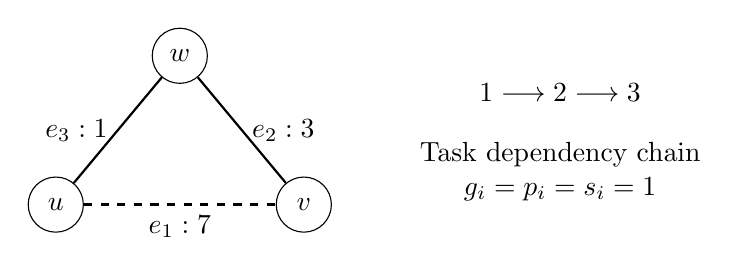
\begin{tikzpicture}[scale=1.05,vertex/.style={circle,draw,minimum size=7mm,inner sep=0pt}]
\node[vertex] (a) at (0,0) {$u$};
\node[vertex] (b) at (3,0) {$v$};
\node[vertex] (c) at (1.5,1.8) {$w$};
\draw[dashed,very thick] (a)--node[below]{$e_1:7$}(b);
\draw[thick] (b)--node[right]{$e_2:3$}(c);
\draw[thick] (a)--node[left]{$e_3:1$}(c);
\node at (6.1,1.35) {$1\longrightarrow 2\longrightarrow 3$};
\node[align=center] at (6.1,0.4) {Task dependency chain\\$g_i=p_i=s_i=1$};
\end{tikzpicture}
\caption{The dashed edge is the retained cut, not a connecting tree edge. The tree minimizes discarded amplification weight. This is a topologically realizable graph example, not a measured native knot input.}\label{fig:triangle}
\end{figure}
Without reuse, $(d_1,d_2,d_3)=(1,1,1)$ and the event bounds are $(1,3,7)$, totaling $11$. Retaining the first candidate gives $(0,1,1)$ and bounds $(0,1,3)$, totaling $4$. Retaining only the last candidate gives $(1,1,0)$ and bounds $(1,3,6)$, totaling $10$. The difference comes from downstream rebuilding, although all three local savings equal one. The supplied example packet reproduces these arithmetic values and the selected tree.

\section{A conditional quasi-polynomial recognition theorem}\label{sec:qp}
\subsection{The structural hypothesis is causal, not just chronological}
Let $n\geq2$ be the input bit length of an authenticated knot diagram or exterior encoding. A persistence implementation may operate in a succession of source epochs, each with a fixed dependency arena. Source epochs are different from the per-task epochs used in Theorem~\ref{thm:causal}: they delimit changes to the task graph or the underlying geometric namespace.

\begin{theorem}[End-to-end accounting under explicit geometric obligations]\label{thm:qp}
Consider a deterministic hierarchy-based recognition implementation satisfying the following conditions on a class $\mathcal C$ of inputs.
\begin{enumerate}[label=(\roman*)]
\item Its geometric transformations and terminal certificates have an independently proved soundness and completeness theorem for unknot recognition on $\mathcal C$. Persistence does not omit any global proof obligation used by that theorem.
\item There are at most $n^{O(1)}$ source epochs. In each epoch there are at most $L=n^{O(1)}$ task slots, rebuild caps $g_i\leq n^{O(1)}$, and a fixed sound acyclic dependency graph of maximum indegree $\Delta\leq n^{O(1)}$ and maximum path length $h=O(\log n)$.
\item All work in an epoch, including initialization, candidate construction, unsuccessful searches, source authentication, pattern transport, task bookkeeping, and terminal checks, is charged either to $n^{O(1)}$ overhead or to its legal version events with per-event bit cost at most $n^{O(\log n)}$. Intermediate encodings satisfy the bounds required for that cost. The implementation cannot perform uncharged infinite or super-budget polling.
\item Retention is permitted only by authentic source-local transport certificates. Rebuilds occur only for genuine changed snapshots, and every repair decreases the charged potential. Creation of new slots or changes to dependencies are included in the source-epoch bounds.
\end{enumerate}
Then the implementation recognizes every input in $\mathcal C$ in bit time $n^{O(\log n)}$.
\end{theorem}
\begin{proof}
By Corollary~\ref{cor:depth}, the event count in one source epoch is at most
\[
 n^{O(1)}\sum_{r=0}^{O(\log n)}(n^{O(1)})^r=n^{O(\log n)}.
\]
Multiply by the assumed per-event bit cost and add the bounded overhead. A product of two quantities of the form $n^{O(\log n)}$ has the same form. Summing over polynomially many source epochs preserves the bound. The termination and verdict are those of the separately sound and complete transformed hierarchy procedure in condition (i); the counting theorem supplies its time bound, not its topological correctness.
\end{proof}

For polynomial per-event costs the same conclusion follows. More generally one can replace the uniform depth condition by the sharper directly evaluated budget
\[
 \sum_i p_i\sum_{P:i_0\leadsto i}d_{i_0}\prod_{v\in P\setminus\{i_0\}}(g_v+1)
 \leq n^{O(\log n)}.
\]
This permits some deep paths whose total weighted contribution is small, for example because their initial progress is already exhausted and no relevant upstream changes occur.

\subsection{What has and has not been achieved}
The theorem isolates a structural route to the requested asymptotic target. It does \emph{not} assume a quasi-polynomial recognizer as a black box: it asks for explicit local encodings, valid transformation rules, charged costs, and a low-depth dependence theorem. These are mathematically separate questions. However, neither this paper nor its reference code proves that arbitrary knot exteriors admit such a persistence implementation.

The native source-map and compressed route exporter are missing from this delivery. A small number of stored surfaces is not established in general; indeed a short initial nonseparating batch cannot be the sole mechanism, by Corollary~\ref{cor:knot-barrier}. Dynamic dependencies may form cycles. Task potentials might increase under normalization. An ostensibly local operation can invalidate global boundary-pattern reasoning. Any one of these failures prevents invoking Theorem~\ref{thm:qp} until it is repaired or quantitatively bounded.

A cap given in a short binary string is not automatically a polynomial \emph{numerical} cap. If $g=2^{n}$, logarithmic causal depth in~\eqref{eq:height} does not yield $n^{O(\log n)}$. Similarly, polynomial-time arithmetic in an exponentially long attaching map is not a polynomial encoded operation. Both quantities must be measured in the stated input model.

\section{Implementation, finite validation, and measurements}\label{sec:implementation}
\subsection{Delivered modules and trust separation}
\code{code/cographic.py} implements graph validation, side-census decoding, Kruskal batch selection, optional signed fundamental cycles, and the finite source routing forest. \code{code/causal.py} implements forward bounds, reverse amplification, a legal-event scheduler, and source-interval overlap predicates. Neither module implements a knot recognizer. \code{code/reuse.py} composes the amplification weights, candidate-to-task injection, and batch optimizer into a single replayable retention plan.

\code{code/verify.py} imports none of the producer modules. It independently checks tree and cycle conditions, reconstructs finite source components with breadth-first search, and replays version histories from snapshots and remaining budgets. Its composite checker also recomputes the amplification weights, saved-progress budgets, and before/after work bounds; it does not trust supplied reward weights to represent the causal objective. This separation detects discrepancies between the producer and verifier algorithms, although it is not a formal proof of the Python runtime or a Lean formalization.

The packet schema explicitly states that a batch is relative to an authenticated chamber graph. The source-routing packet claims only finite-arena semantics. There is no field named ``unknot certificate'' and no implicit conversion to a recognition verdict. Malformed data are rejected; a scheduler event limit stops execution without declaring a completed history.

\subsection{Completed finite checks}
The supplied run used CPython 3.13.5 on Linux. All 17 test methods passed with no failures, errors, or skips. The recorded elapsed time was approximately 2.61 seconds; this is an environment-specific suite measurement, not a complexity estimate. The full counts are in \code{results/validation.json}.

\begin{center}\small
\begin{tabular}{lr}
\toprule
Completed check family & Count\\
\midrule
Connected simple graphs on one through five vertices & 772\\
Subset connectivity and binary rank identities & 55,895\\
Signed fundamental graph cycles & 1,259\\
All marker partitions for $k=0,\ldots,4$ & 4,361\\
Accepted connected side partitions among those & 2,608\\
Weighted multigraphs checked against all subsets & 320\\
Independent rational-rank checks & 240\\
Finite source arenas / lifted fundamental cycles & 450 / 1,797\\
DAG recurrences compared with literal path sums & 1,500\\
Random legal histories / their events & 600 / 7,622\\
Partial-progress DAGs / their replayed events & 450 / 65,774\\
Sharp chain instances / their events & 18 / 9,078\\
Amplified optimal-reuse problems checked exhaustively & 180\\
Eventwise potential histories / checked events & 400 / 4,139\\
Tampered packets / illegal histories rejected & 816 / 7\\
Largest integer bit length exercised & 16,385\\
\bottomrule
\end{tabular}
\end{center}

The connectivity oracle uses independent adjacency traversal, not the producer's disjoint-set structure. The weighted oracle enumerates every candidate subset on the sampled small instances. Rational elimination is separate from binary row reduction. The path-sum oracle literally enumerates directed paths on small DAGs, whereas the implementation evaluates a recurrence. Tests for partial progress compare both the forward/reverse work identity and independently replayed scheduler histories.

The large-integer tests use huge weights and source ranks without iterating to those ranks. They demonstrate binary arithmetic behavior in these modules. They do not test the missing compressed geometric path exporter or the AHT implementation. No native ProveIt test suite, Regina geometry, maintained recognizer, or knot benchmark was run here.

\subsection{Paired graph-stage benchmark}
Both measured arms start from the same already supplied side histogram and rewards. They decode it, solve the same weighted batch problem, construct a certificate, and run the same independent checker. The new arm uses spanning-tree optimization. The reference arm enumerates all $2^k$ candidate subsets. It is an exhaustive mathematical baseline, \emph{not} a claim about the algorithm previously used by ProveIt.

For each case, one untimed call of each method precedes seven shuffled paired rounds. An identical exhaustive arm supplies a control. Tiny cases use 500 calls per sample, the eight-edge case uses 20, and larger cases use one. All 168 arm samples finish, and all objective values and certificates agree. Imports and input fixture generation are excluded. There is no weighted-orbit producer cost in either arm because the census is the given input to this comparison.

\begin{table}[ht]
\centering\small
\begin{tabular}{lrrrrr}
\toprule
Case & $k$ & New (ms) & Exhaustive (ms) & Ratio & Control \\
\midrule
empty & 0 & 0.0042 & 0.0041 & 0.98 & 0.992 \\
one\_loop & 1 & 0.0069 & 0.0074 & 1.06 & 0.990 \\
parallel\_pair & 2 & 0.0092 & 0.0111 & 1.21 & 1.011 \\
triangle & 3 & 0.0115 & 0.0177 & 1.54 & 1.014 \\
bouquet\_8 & 8 & 0.0181 & 0.4196 & 23.07 & 1.005 \\
multi\_5\_10 & 10 & 0.0404 & 2.2359 & 61.36 & 0.998 \\
multi\_6\_14 & 14 & 0.0794 & 42.2618 & 534.84 & 1.017 \\
multi\_7\_18 & 18 & 0.0913 & 804.9267 & 8761.54 & 0.997 \\
\bottomrule
\end{tabular}
\caption{Complete graph-stage calls, including certificate replay. Ratio is the median paired exhaustive/new ratio; control is the median identical exhaustive-control/exhaustive ratio. These are local graph-query measurements, not recognition gains.}\label{tab:benchmark}
\end{table}

The largest case illustrates the expected removal of subset enumeration, but its large ratio must not be advertised as an unknot speedup. The empty case shows a small regression, and the tiny controls show measurable timing variation. Most of the asymptotic gain in this table follows from replacing an exponential reference search by a classical polynomial graph algorithm. The more distinctive algorithmic question is whether source-authenticated causal rewards select materially better reusable work inside a real hierarchy; these measurements do not answer it.

\subsection{Execution-count experiments versus running-time claims}
The sharp-chain tests realize the exact version counts in~\eqref{eq:sharp}; the independent-task tests realize additive counts. These are complete executions of the abstract scheduler. The additional eventwise tests verify the potential decrease, including unobserved-parent debts, along independently replayable randomized histories. They validate that rebuild events are being counted and that the claimed exponential example is not just an overestimate in that model. They neither construct a worst-case knot family nor establish that a real hierarchy can replace a chain by an antichain.

\section{A proposed native integration contract}\label{sec:integration}
\subsection{Producer boundary}
The first native adapter should consume the maintained raw-cut packet and produce the following \emph{source-authenticated} data: labeled connected candidate components with coherent sides; the chamber-equivalence instance; one marked atom per side; the weighted census and its independent proof; and the source identity used by every marker. The graph decoder then requires no geometric heuristics.

The second adapter should export a shared route grammar, not expanded paths through every parallel copy. Its checker must reconstruct each graph-level step in the source, certify the unique selected-surface crossing, and provide conservative read supports. If a loop description is compressed but its read support expands exponentially, it does not yet support the proposed persistence optimizer.

\subsection{Transaction boundary}
A candidate retention transaction should not commit piecemeal. It should verify the source identity, all relevant source certificates, the graph batch certificate, the route witnesses, and the edit/transport proof. Then it can update the task snapshot atomically. An incomplete or timed-out transaction leaves the prior validated state intact, or marks the affected tasks stale without using their results.

The DAG contains real \emph{validity} dependencies, not merely computational call relationships. A proof that uses an ambient boundary-pattern fact must depend on the certificate establishing that fact. Shared source labels need explicit versioning after quotient or re-embedding operations; retaining the same integer index is not evidence that the same geometric cell survives.

\subsection{Scheduling policy}
Use reverse amplification scores to order bounded attempts or select an authentic valid batch. Recompute the scores when a new source epoch legitimately changes the dependency graph. Do not adaptively remove dependencies merely to improve the displayed bound. For a conservative dependency graph, extra edges can worsen performance but not soundness; missing edges can corrupt a verdict.

No automatic recognition dispatch change is proposed in this bundle. A first integration can expose a research-only command that produces and replays batch packets while the existing recognizer continues unchanged. Full paired measurements should separately include candidate generation, both source adapters, verification, retained work, failed attempts, and the fallback cost. A local graph-stage ratio is not an adequate substitute.

\section{Further research questions and concrete next milestones}\label{sec:future}
\subsection{Source geometry and compressed witnesses}
\paragraph{Q1. A native labeled-batch exporter.}
Can the maintained raw-cut families authenticate connected cooriented surface components and one side marker each without expanding normal multiplicities? The initial target should include a single nonseparating surface, parallel meridian disks, loops and parallel edges in the chamber graph, and a rejection case with a one-sided component. This is the smallest meaningful bridge from the current repository to Theorem~\ref{thm:census}.

\paragraph{Q2. Orbit proofs that carry return routes.}
Can the weighted-orbit reduction trace be augmented with a straight-line or interval grammar for paths between selected source atoms? Prove a polynomial bound on grammar size \emph{and} on checking that its interpretation stays within one chamber. Endpoint membership alone is insufficient.

\paragraph{Q3. A compressed read-support calculus.}
For a route grammar, can one compute a conservative union of source incidences that it reads, with size polynomial in the grammar? Arbitrary unions of affine path supports may fragment. A useful theorem would identify a stable family closed under concatenation, inversion, and the actual source cuts used by the repository.

\paragraph{Q4. Sharing without destructive aliasing.}
When many dual loops use a common routing subtree, can an edit be checked once against that shared subtree and its dependent witnesses invalidated efficiently? The graph-level tree supports this optimization, but source-chart transport must preserve its semantics under re-embedding.

\subsection{The geometric origin of small causal depth}
\paragraph{Q5. Persistence of the actual hierarchy obligations.}
Classify which compression, pattern-compression, admissibility, and parallelity operations have sound local transport theorems for \emph{all} properties their descendants need. Nonseparation is only the first such property. A useful negative result would exhibit an unavoidable long-range dependency despite disjoint surface supports.

\paragraph{Q6. A low-depth normal form or a barrier family.}
Does every relevant hierarchy admit a source-authenticated schedule with polynomially bounded caps and $O(\log n)$ actual causal depth? Alternatively, construct a family forcing superlogarithmic dependency depth for this specific certificate language. A chronological length bound alone would not settle either direction.

\paragraph{Q7. What replaces initial parallelism?}
Corollary~\ref{cor:knot-barrier} rules out a large initial nonseparating batch. Can an early certified cut create later independent subproblems whose certificates remain local under upstream repair? Quantify how their first homology and source-interface sizes develop, instead of assuming that every cut supplies more reusable freedom.

\paragraph{Q8. Dynamic dependency arenas.}
Can changing task sets be handled by a controlled refinement of a fixed master DAG? Prove bounds on births and source epochs, or derive a potential charging new dependencies to decreases in q-complexity. Corollary~\ref{cor:injection} supplies a precise alternative: bound the total injected causal potential and separately charge the actual arena-switch work. Unbounded graph rebuilding would otherwise defeat the fixed-arena bounds even when every individual graph has small depth.

\subsection{Sharper optimization and event accounting}
\paragraph{Q9. Coalescence-aware path bounds.}
The path recurrence can overcount when a task has several simultaneously stale parents. Can one retain an equally checkable bound that recognizes joint invalidations without exponential state? Chains are already sharp, so any improvement must use actual merging structure rather than merely replace $g_i+1$ by $g_i$.

\paragraph{Q10. Beyond additive retention rewards.}
Source sharing can make the cost of retaining two surfaces subadditive or superadditive. Characterize useful reward classes for which cographic feasibility still permits polynomial-time optimal reuse, or isolate approximation guarantees with a rigorous upper-bound interpretation. Theorem~\ref{thm:combined} deliberately requires additive initial-progress savings.

\paragraph{Q11. Optimizing geometry and dependencies together.}
Different chamber spanning trees produce different return routes. The present objective assumes a fixed downstream DAG, but choosing a tree may alter route overlap and therefore future dependencies. Can one optimize a coupled tree-and-support objective while retaining independent verification? This is a natural point where the simple minimum-spanning-tree solution may cease to suffice.

\paragraph{Q12. Numeric potential bounds after compression.}
Prove a polynomial bound in the original input on the \emph{numerical} rebuild caps of a useful source-local task decomposition. Encoded normal coordinates may be exponentially large while pattern complexity is small; identify exactly which geometric reductions maintain the latter without expanding the former.

\subsection{Verification and empirical discrimination}
\paragraph{Q13. Native counterexample-driven validation.}
Implement the parallel-meridian obstruction in the actual source format and require the retention layer to reject the pair while accepting either singleton. Add a case where an edit misses a surface but hits its dual route. These tests specifically distinguish correct persistence from surface-only caching.

\paragraph{Q14. Paired whole-hierarchy measurements.}
Compare suffix discard, conservative proof-support invalidation, and amplification-weighted retention on identical source inputs and budgets. Record total candidates, actual version changes, source verification time, encoding sizes, and maximum causal depth. A null result or regression would identify the next bottleneck more reliably than increasing a local graph benchmark size.

\paragraph{Q15. Formalization of the small trusted core.}
Formalize the graph connectivity equivalence, the fundamental-cycle identity certificate, the snapshot charging argument, and the reverse amplification identity. These finite statements are suitable early targets. Their formalization should not be described as a formalization of the native source geometry until the adapter's semantic theorem is also supplied.

\paragraph{A focused next experiment.}
The highest-value next deliverable is a native, source-authenticated export of a small chamber graph plus a replayable dual route for one candidate. Once its conservative read support survives an actual local edit, the first real dependency edges can be measured. That evidence would directly test the central hypothesis behind the new reset bound, rather than only its already verified abstract arithmetic.

\section{Conclusion}
A hierarchy's restart cost is not determined solely by how many surfaces it stores. It depends on which certified work genuinely becomes invalid and on how that invalidation propagates. The chamber graph gives an exact, small optimizer for simultaneous nonseparation. Dual loops supply transportable witnesses with explicit local hypotheses. The version model turns genuine dependencies into a weighted path bound, and its reverse recurrence gives mathematically justified retention rewards.

These results solve well-defined subproblems and expose a sharper route to $n^{O(\log n)}$ accounting: small \emph{causal} depth with controlled source operations. They also identify concrete barriers, including the one-dimensional first homology of an initial knot exterior and the insufficiency of connectivity histograms as geometric path certificates. The general recognition objective now requires source-authenticated realization and a global structural theorem, not a reinterpretation of the finite tests as an end-to-end proof.

\appendix
\section{Proof audit and edge cases}\label{app:audit}
\paragraph{Connectedness of the candidates is indispensable.}
A disconnected surface can have several negative-side chambers and several positive-side chambers. Encoding it by one edge loses information. The correct repair is to authenticate and label its connected components before using this paper's graph interface; giving one arbitrary marker to the entire disconnected union is not valid.

\paragraph{Coorientation is indispensable to the stated integral model.}
A one-sided surface does not have two globally separated collar sides. The two-side marker scheme and the signed one-crossing certificate are not its correct representation. An orientation-cover approach may be possible but is not silently included in these theorems.

\paragraph{Individual versus simultaneous witnesses.}
Each of two parallel meridians has a closed loop crossing it once. No two such loops can satisfy the cross-avoidance condition for the pair, because its two cohomology classes are dependent. Thus storing individual nonseparation verdicts is weaker than storing a batch certificate.

\paragraph{Not every retained fact is source-local.}
Theorem~\ref{thm:persistence} preserves a positive witness. It does not prove that there is no compression disk elsewhere. Global absence statements require different proof objects or transport arguments. This prevents a common unsound inference from ``none of the surface's cells changed'' to ``all its old hierarchy obligations remain true.''

\paragraph{Zero-potential tasks can still cost work.}
A task with $g_i=0$ makes no repairs but may rebuild after each parent change. Its recurrence is $B_i=\sum_{j\to i}B_j$, not zero. This is why the coefficient is $g_i+1$. If every initial budget is zero and no exogenous source event occurs, then all $B_i$ are zero and there is no legal version event at all.

\paragraph{A cycle is not a DAG.}
The proof charges events in topological order. Repeated mutually invalidating tasks cannot be inserted into the same argument. They must be grouped into a separately bounded transaction or controlled by an independent potential. A graph with a directed cycle is rejected by the current topological-ID input contract.

\paragraph{Initialization and newly created tasks.}
The event counts begin with all snapshots valid. Building them is charged separately. A program that repeatedly throws away the whole arena and starts over has not violated an individual arena bound, but it has created more source epochs. Those epochs must be controlled in any use of Theorem~\ref{thm:qp}.

\paragraph{Reward optimality has a fixed comparison class.}
The combined theorem compares authentic valid batches under the same dependency graph, costs, and rebuild caps. If the chosen route changes those quantities, they must be re-evaluated; the earlier objective is no longer the same objective. Nor is minimizing a rigorous upper bound the same as minimizing actual wall-clock time.

\section{Reproduction and source audit}\label{app:reproduction}
From the package root, use:
\begin{lstlisting}
python tests/test_research.py
python code/demo.py
python code/benchmark.py
sh build.sh
\end{lstlisting}
The test program writes a structured validation record. The benchmark writes all raw paired samples and regenerates its LaTeX table. The demo emits a batch certificate, a finite-routing packet, and a sharp-chain history. All Python modules use only the standard library. Building the article needs a conventional LaTeX installation with the packages declared in its preamble.

The repository branch was inspected at commit
\begin{quote}\small\ttfamily
704600626606a9097cfd89d4e3d2bbc63c8dd1cb.
\end{quote}
The raw-cut article was explicitly fetched at that commit, with blob
\begin{quote}\small\ttfamily
dc12b1a58aedaed78f00b63109b0aa5214832ca1.
\end{quote}
Other initial documentation reads used the then-current branch without a commit argument; their returned blob identifiers are recorded separately in \code{SOURCE_AUDIT.md}. The study did not obtain or execute a full native checkout. Incoming directory metadata were inspected, and related individual manuscript excerpts were retrieved from the user's Library. The complete incoming ZIP contents were not all read. This is a targeted continuation, not a claim of an exhaustive audit of every contemporaneous report.

\section{Claim and evidence ledger}
\small
\begin{longtable}{p{0.43\textwidth}p{0.51\textwidth}}
\toprule
Claim & Status and evidence\\
\midrule\endhead
Integral chamber-cycle and subbatch theorems & Proved in Section~\ref{sec:duality}; classical foundations made explicit. Finite graph rank checks corroborate the algebra.\\
One scalar chamber census & Proved in Theorem~\ref{thm:census}, conditional on authentic side markers and chamber relation. Weighted census algorithm imported; native exporter not implemented.\\
Optimal weighted batch & Proved in Theorem~\ref{thm:mst}; implemented and compared with exhaustive search.\\
Disjoint dual-loop existence & Proved topologically in Theorem~\ref{thm:loops}; geometric disjointification is not implemented.\\
Shared finite routing forest & Proved in Proposition~\ref{prop:routing}; implemented with independent finite replay. Not a binary source-path exporter.\\
Local persistence of nonseparation & Proved in Theorem~\ref{thm:persistence} under unchanged-neighborhood or surgery hypotheses. No assertion of automatic global admissibility.\\
Causal reset path bound & Proved in Theorems~\ref{thm:causal}--\ref{thm:paths}; exact on tested chain executions.\\
Eventwise potential and arena-switch injections & Proved in Theorem~\ref{thm:potential} and Corollary~\ref{cor:injection}; 4,139 eventwise checks on 400 histories.\\
Downstream-amplified optimal reuse & Proved in Theorem~\ref{thm:combined}; 180 small coupled instances checked exhaustively under fixed dependencies.\\
Initial large nonseparating knot batch & Ruled out: Corollary~\ref{cor:knot-barrier} bounds its size by one.\\
Graph-stage speedup & Measured against a defined exhaustive reference with replay and paired controls. Not an upstream benchmark.\\
General quasi-polynomial recognition & Not established. Theorem~\ref{thm:qp} states sufficient geometric, causal, and encoded-cost conditions.\\
Native integration and full regression & Not performed. Proposed contract and next experiments appear in Section~\ref{sec:integration}.\\
\bottomrule
\end{longtable}
\normalsize

\begin{thebibliography}{10}
\addcontentsline{toc}{section}{References}
\bibitem{lackenby}
M.~Lackenby, \emph{Incompressible surfaces, hierarchies and unknot recognition}, arXiv:2607.23350v1, 25 July 2026. Targeted reading: Sections~6, 8--10, and the hierarchy interfaces.
\url{https://arxiv.org/abs/2607.23350}.

\bibitem{aht}
I.~Agol, J.~Hass, and W.~Thurston, \emph{The computational complexity of knot genus and spanning area}, arXiv:math/0205057v2. Theorem~12 gives interval-orbit counting and Theorem~16 gives its weighted form.
\url{https://arxiv.org/abs/math/0205057}.

\bibitem{repo}
ProveIt contributors, \emph{Unknot recognition project README}, \code{Topology/UnknotRecognition/README.md}, inspected 12 October 2026. Source scope and returned blob recorded in \code{SOURCE_AUDIT.md}.
\url{https://github.com/VladimirReshetnikov/ProveIt/tree/main/Topology/UnknotRecognition}.

\bibitem{cutcells}
ProveIt contributors, \emph{Full three-dimensional normal cuts in affine cell families}, \code{Topology/UnknotRecognition/synthesis/cut_cells.tex}, at commit \code{704600626606a9097cfd89d4e3d2bbc63c8dd1cb}, 2026.
\url{https://github.com/VladimirReshetnikov/ProveIt/blob/704600626606a9097cfd89d4e3d2bbc63c8dd1cb/Topology/UnknotRecognition/synthesis/cut_cells.tex}.

\bibitem{moment}
Research continuation prepared for ProveIt, \emph{Moment-coded first returns}, 12 October 2026. Individual manuscript's scope and evidence ledger inspected via the user's Library; incoming archive \code{ProveIt_Moment_Coded_First_Returns_2026-10-12.zip}.

\bibitem{corners}
Research continuation prepared for ProveIt, \emph{Corner-Aware Boundary Kernels for Compressed Unknot Hierarchies: Exact port surgery, orbit-count compilation, and interval-bundle consequences}, 12 October 2026. Individual manuscript abstract and scope inspected via the user's Library.

\bibitem{sparse}
Research continuation prepared for ProveIt, \emph{Sparse Cut Grammars}, 12 October 2026. Related incoming manuscript and bibliographic scope; not used as a black-box theorem in this paper.

\bibitem{closures}
ProveIt contributors, \emph{Classical closures, first jets, and bounded diagram resets}, \code{Topology/UnknotRecognition/synthesis/closure_resets.tex}, inspected 12 October 2026.
\url{https://github.com/VladimirReshetnikov/ProveIt/blob/main/Topology/UnknotRecognition/synthesis/closure_resets.tex}.

\bibitem{causalr3}
Research continuation prepared for ProveIt, \emph{Causal-Branch Parameterization of Reidemeister-III Unlocking}, Report~25, 7 October 2026. Individual manuscript's theorem statements and hierarchy-transfer discussion inspected via the user's Library. This concerns diagram rewriting, not the version model developed here.
\end{thebibliography}
\end{document}
